\documentclass[12pt]{article}
\usepackage{amsmath, amssymb}
\usepackage{graphicx}
\usepackage{xcolor}
\usepackage{hyperref}
\usepackage{physics}
\usepackage{tikz}
\usepackage{booktabs}
\usetikzlibrary{quantikz}

\title{Quantum Mechanics Fundamentals for Quantum Computing}
\author{Quantum Computing Course}
\date{Lecture Notes}

\begin{document}

\maketitle

\section*{Lecture Overview}
\textbf{Duration:} 1.5 hours \\
\textbf{Objective:} Provide intuitive understanding of quantum mechanical concepts essential for quantum computing, emphasizing connections to computation rather than mathematical formalism.

\section{Introduction: Why Quantum Mechanics for Computer Scientists?}

\subsection{The Classical vs Quantum World}
\begin{itemize}
    \item Classical computers: Bits as definite states (0 or 1)
    \item Quantum computers: Qubits as probabilistic, superposition states
    \item Analogy: Classical probability vs Quantum probability amplitudes
    \item Key insight: Quantum mechanics provides new computational primitives
\end{itemize}

\section{Wave-Particle Duality}

\subsection{The Double-Slit Experiment}

\begin{figure}[h]
    \centering
    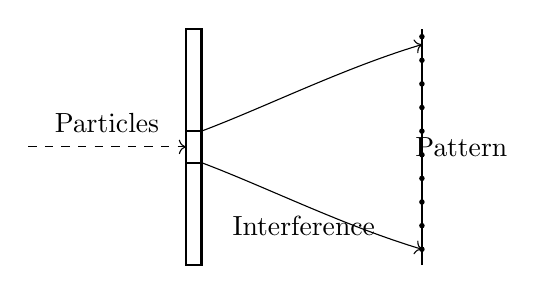
\begin{tikzpicture}
        % Double slit diagram
        \draw[thick] (0,0) rectangle (0.2,3);
        \draw[thick] (0,1.3) -- (0.2,1.3);
        \draw[thick] (0,1.7) -- (0.2,1.7);
        \draw[dashed,->] (-2,1.5) -- (0,1.5);
        \draw[->] (0.2,1.3) .. controls (1,1) and (2,0.5) .. (3,0.2);
        \draw[->] (0.2,1.7) .. controls (1,2) and (2,2.5) .. (3,2.8);
        \draw[thick] (3,0) -- (3,3);
        \foreach \y in {0.2,0.5,0.8,1.1,1.4,1.7,2.0,2.3,2.6,2.9} {
            \fill (3,\y) circle (1pt);
        }
        \node at (-1,1.8) {Particles};
        \node at (1.5,0.5) {Interference};
        \node at (3.5,1.5) {Pattern};
    \end{tikzpicture}
    \caption{Double-slit experiment showing wave-like interference patterns}
\end{figure}

\subsubsection{Experimental Setup}
\begin{itemize}
    \item Particles (electrons/photons) sent through two slits
    \item Classical expectation: Two bands on detection screen
    \item Quantum reality: Interference pattern emerges
\end{itemize}

\subsubsection{Key Observations}
\begin{enumerate}
    \item \textbf{With both slits open:} Interference pattern (wave-like behavior)
    \item \textbf{With measurement:} Which-path information destroys interference
    \item \textbf{Single particles:} Even single particles show interference over time
\end{enumerate}

\subsubsection{Connection to Quantum Computing}
\begin{itemize}
    \item Quantum states can exist in multiple paths simultaneously
    \item Measurement collapses possibilities to definite outcomes
    \item Basis for quantum parallelism
\end{itemize}

\section{Quantum Superposition: Physical Meaning}

\subsection{Conceptual Idea}

In classical computing, a bit is always in one of two definite states:
\[
0 \quad \text{or} \quad 1.
\]

In quantum mechanics, physical systems can be prepared in states that are not associated with a single definite outcome.
Instead, the system is described by a \emph{quantum state} that encodes multiple possible outcomes simultaneously.

\textbf{Important:}
Superposition does \emph{not} mean that a system secretly has multiple values at once.
It means the system is in a single physical state whose measurement outcomes are not predetermined.

\begin{figure}[h]
    \centering
    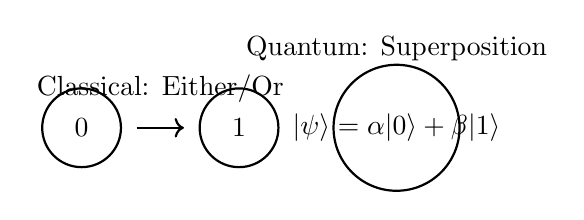
\begin{tikzpicture}
        % Classical vs Quantum comparison
        \draw[thick] (0,1.5) circle (0.5) node {0};
        \draw[thick] (2,1.5) circle (0.5) node {1};
        \draw[->, thick] (0.7,1.5) -- (1.3,1.5);
        \node at (1,2) {Classical: Either/Or};
        
        \draw[thick] (4,1.5) circle (0.8);
        \draw (4,1.5) node {$|\psi\rangle = \alpha|0\rangle + \beta|1\rangle$};
        \node at (4,2.5) {Quantum: Superposition};
    \end{tikzpicture}
    \caption{Classical vs Quantum state representation}
\end{figure}

\subsection{Mathematical Representation (Preview)}

A qubit state is represented by a vector:
\[
|\psi\rangle = \alpha |0\rangle + \beta |1\rangle,
\]
where $\alpha, \beta \in \mathbb{C}$ are probability amplitudes satisfying
\[
|\alpha|^2 + |\beta|^2 = 1.
\]

Probabilities arise only upon measurement:
\[
P(0) = |\alpha|^2, \quad P(1) = |\beta|^2.
\]

The complex nature of $\alpha$ and $\beta$ allows for \emph{interference} effects, which are crucial for quantum computation.

\subsection{Creating Superposition in Physical Systems}

\subsubsection{Coherent Excitation of Atomic Systems}

Electrons in atoms do not follow classical orbits. Instead, they occupy quantum energy eigenstates. The energy levels are quantized, meaning electrons can only exist in specific discrete energy states.

Carefully controlled interactions (e.g., laser pulses) can prepare coherent superpositions such as:
\[
|\psi\rangle = \frac{1}{\sqrt{2}} (|g\rangle + |e\rangle).
\]

The laser pulse duration and frequency must be precisely tuned to create equal superpositions (known as $\pi/2$ pulses). The phase relationship between $|g\rangle$ and $|e\rangle$ is preserved during this process.

\textbf{Key Challenge:} Uncontrolled interactions with the environment destroy such superpositions, a process known as \emph{decoherence}. This is one of the main obstacles in building quantum computers.

\subsubsection{Photonic Superposition}

Photons are particularly useful because they interact weakly with their environment, making them less susceptible to decoherence.

Examples include:
\begin{itemize}
    \item \textbf{Polarization superpositions:}
    \[
    |\psi\rangle = \frac{1}{\sqrt{2}}(|H\rangle + |V\rangle),
    \]
    created using waveplates that rotate polarization states.
    
    \item \textbf{Path superpositions:} Created by beam splitters that partially transmit and partially reflect photons. A single photon incident on a 50/50 beam splitter becomes:
    \[
    |\psi\rangle = \frac{1}{\sqrt{2}}(|\text{transmitted}\rangle + |\text{reflected}\rangle).
    \]
    
    \item \textbf{Phase superpositions:} Using interferometers to create superpositions with different phase relationships.
\end{itemize}

In all cases, the photon is never split into pieces—only its \emph{state} is delocalized. This is a crucial distinction: we're creating superposition of possible measurement outcomes, not dividing the particle itself.

\subsection{Visualizing Superposition: Bloch Sphere}
\begin{figure}[h]
    \centering
    \begin{tikzpicture}[scale=1.5]
        % Bloch Sphere
        \draw (0,0) circle (2cm);
        \draw[->] (0,-2.5) -- (0,2.5) node[above] {$z$};
        \draw[->] (-2.5,0) -- (2.5,0) node[right] {$x$};
        \draw[->] (0,0) -- (1.414,1.414) node[above right] {$y$};
        \draw[dashed] (0,0) -- (1.5,1.5);
        \node at (0,2.2) {$|0\rangle$};
        \node at (0,-2.2) {$|1\rangle$};
        \node at (2.2,0) {$|+\rangle = \frac{|0\rangle+|1\rangle}{\sqrt{2}}$};
        \node at (-2.2,0) {$|-\rangle = \frac{|0\rangle-|1\rangle}{\sqrt{2}}$};
        \fill (1.5,1.5) circle (2pt) node[right] {$|\psi\rangle$};
        \draw[->] (0,0) -- (1.5,1.5);
        \draw (0.5,0) arc (0:45:0.5);
        \node at (0.7,0.3) {$\theta$};
    \end{tikzpicture}
    \caption{Bloch sphere representation of a qubit. Any point on the sphere represents a valid qubit state. The poles represent classical states, while points on the equator represent equal superpositions with different phases.}
\end{figure}

\begin{itemize}
    \item North pole: $|0\rangle$ (classical 0)
    \item South pole: $|1\rangle$ (classical 1)
    \item Equator: Equal superpositions $\frac{1}{\sqrt{2}}(|0\rangle + e^{i\phi}|1\rangle)$
    \item Any point on sphere: Valid qubit state with specific superposition weights and relative phase
\end{itemize}

\section{Measurement and Quantum Probability}

Measurement is an active physical process that extracts classical information from a quantum system. Unlike classical measurement which reveals a pre-existing property, quantum measurement fundamentally changes the system.

The measurement postulate states that when we measure a quantum state $|\psi\rangle$ in a basis $\{|i\rangle\}$, the probability of outcome $i$ is:
\[
P(i) = |\langle i | \psi \rangle|^2.
\]

After measurement, the system \emph{collapses} to the corresponding basis state:
\[
|\psi\rangle \xrightarrow{\text{measure } i} |i\rangle.
\]

\textbf{Crucial properties:}
\begin{enumerate}
    \item \textbf{Irreversibility:} Measurement destroys coherence with respect to the measurement basis
    \item \textbf{Probabilistic:} Outcomes are fundamentally random (not due to ignorance)
    \item \textbf{Basis-dependent:} Different measurement bases yield different probability distributions
    \item \textbf{Repeatability:} Immediate re-measurement gives the same result
\end{enumerate}

\subsection{Multiple Measurement Bases}
\begin{itemize}
    \item \textbf{Computational basis:} $\{|0\rangle, |1\rangle\}$ - measures "classical" value
    \item \textbf{Hadamard basis:} $\{|+\rangle, |-\rangle\}$ where $|\pm\rangle = \frac{1}{\sqrt{2}}(|0\rangle \pm |1\rangle)$
    \item \textbf{General basis:} Any orthonormal set of vectors
\end{itemize}

The choice of measurement basis is equivalent to asking different questions about the quantum system.

\section{The Uncertainty Principle (Conceptual)}

The uncertainty principle states that certain pairs of observables cannot be simultaneously well-defined. The most famous is the position-momentum uncertainty relation:
\[
\Delta x \cdot \Delta p \geq \frac{\hbar}{2}.
\]

This is not due to experimental limitations, but arises from the mathematical structure of quantum states. It reflects the wave-like nature of quantum particles.

\subsection{Physical Interpretation}
\begin{itemize}
    \item A quantum state sharply localized in position ($\Delta x$ small) must necessarily involve a wide range of momenta ($\Delta p$ large)
    \item Conversely, a state with definite momentum ($\Delta p$ small) must be spread out in position ($\Delta x$ large)
    \item This explains why classical trajectories don't exist at the quantum scale
\end{itemize}

\subsection{Computational Analogy}
In quantum computing, we have uncertainty relations between non-commuting observables like:
\begin{itemize}
    \item $X$ (bit-flip) and $Z$ (phase-flip) measurements
    \item The uncertainty principle explains why we cannot simultaneously know both the computational value and phase of a qubit
    \item This has practical implications for quantum error correction and cryptography
\end{itemize}

\subsection{Relevance to Quantum Computing}
\begin{itemize}
    \item \textbf{No-cloning theorem:} You cannot copy an unknown quantum state, a direct consequence of the linearity of quantum mechanics and related to uncertainty principles
    \item \textbf{Quantum cryptography:} Security of protocols like BB84 relies on the fact that measuring one observable disturbs complementary observables
    \item \textbf{Quantum error correction:} Must work around the fact that we cannot measure quantum information without disturbing it
\end{itemize}

\section{Quantum Evolution and Computation}

Between measurements, quantum states evolve deterministically according to the Schrödinger equation:
\[
i\hbar \frac{\partial}{\partial t} |\psi(t)\rangle = \hat{H} |\psi(t)\rangle.
\]

This evolution has several important properties:

\subsection{Properties of Quantum Evolution}
\begin{enumerate}
    \item \textbf{Unitary:} Evolution preserves the norm (total probability = 1)
    \item \textbf{Reversible:} Every transformation has an inverse
    \item \textbf{Linear:} Superpositions evolve independently
    \item \textbf{Deterministic:} Given initial state and Hamiltonian, future state is completely determined
\end{enumerate}

The solution can be written using the time evolution operator:
\[
|\psi(t)\rangle = U(t)|\psi(0)\rangle, \quad \text{where } U(t) = e^{-i\hat{H}t/\hbar}.
\]

\subsection{Connection to Quantum Computing}
In quantum computing:
\begin{itemize}
    \item \textbf{Unitary evolutions} correspond to quantum gates
    \item \textbf{Computation occurs} through controlled interference of probability amplitudes
    \item \textbf{Measurement extracts} classical information at the end
    \item \textbf{The Hamiltonian $\hat{H}$} is engineered to implement desired quantum operations
\end{itemize}

\subsubsection{Example: Quantum Gates as Unitary Operations}
\begin{itemize}
    \item Hadamard gate: Creates superposition
    \[
    H = \frac{1}{\sqrt{2}}\begin{pmatrix} 1 & 1 \\ 1 & -1 \end{pmatrix}
    \]
    \item Pauli-X gate (quantum NOT):
    \[
    X = \begin{pmatrix} 0 & 1 \\ 1 & 0 \end{pmatrix}
    \]
    \item All quantum gates must be unitary: $U^\dagger U = I$
\end{itemize}

\subsubsection{Key Difference from Classical Computing}
\begin{table}[h]
    \centering
    \begin{tabular}{|p{0.45\textwidth}|p{0.45\textwidth}|}
    \hline
    \textbf{Classical Computing} & \textbf{Quantum Computing} \\
    \hline
    Irreversible operations (AND, OR) & All operations reversible (except measurement) \\
    Definite states & Superposition states \\
    No interference & Constructive/destructive interference \\
    Independent bits & Entangled qubits \\
    \hline
    \end{tabular}
    \caption{Fundamental differences between classical and quantum computing}
\end{table}

\section{Entanglement: "Spooky Action at a Distance"}

\subsection{EPR Paradox and Bell States}
Einstein, Podolsky, and Rosen (1935) pointed out that quantum mechanics predicts correlations between distant particles that seem to violate locality. These are now called \emph{entangled states}.

Bell states are maximally entangled two-qubit states:
\begin{align*}
|\Phi^+\rangle &= \frac{1}{\sqrt{2}}(|00\rangle + |11\rangle) \\
|\Phi^-\rangle &= \frac{1}{\sqrt{2}}(|00\rangle - |11\rangle) \\
|\Psi^+\rangle &= \frac{1}{\sqrt{2}}(|01\rangle + |10\rangle) \\
|\Psi^-\rangle &= \frac{1}{\sqrt{2}}(|01\rangle - |10\rangle)
\end{align*}

In these states, the individual qubits don't have definite states, but the pair has definite correlations.

\subsection{Importance for Quantum Computing}
\begin{itemize}
    \item \textbf{Resource for quantum speedup:} Many quantum algorithms rely on entanglement
    \item \textbf{Enables quantum teleportation:} Transfer of quantum states using entanglement and classical communication
    \item \textbf{Essential for quantum error correction:} Encodes logical qubits across multiple physical qubits
    \item \textbf{Basis for quantum cryptography:} Provides security through quantum correlations
\end{itemize}

\section{From Quantum Physics to Quantum Computation}

\subsection{Key Transitions}
\begin{table}[h]
    \centering
    \begin{tabular}{|l|l|}
    \hline
    \textbf{Quantum Mechanics} & \textbf{Quantum Computing} \\
    \hline
    State vector $|\psi\rangle$ & Qubit state \\
    Superposition & Quantum parallelism \\
    Measurement & Readout of computation \\
    Unitary evolution & Quantum gates/circuits \\
    Entanglement & Quantum correlation resource \\
    Uncertainty principle & Limits on information extraction \\
    \hline
    \end{tabular}
    \caption{Bridge between physics and computation}
\end{table}

\subsection{Physical Implementations Overview}
\begin{itemize}
    \item \textbf{Superconducting qubits:} Artificial atoms in circuits (used by IBM, Google)
    \item \textbf{Trapped ions:} Atomic energy levels (used by IonQ, Honeywell)
    \item \textbf{Photonics:} Polarization or path encoding (used by Xanadu, PsiQuantum)
    \item \textbf{Topological qubits:} Anyons (future technology, Microsoft's approach)
\end{itemize}

Each implementation faces different challenges in creating, maintaining, and measuring superpositions.

\section{Practical Examples}

\subsection{Example 1: Quantum Random Number Generator}
\begin{itemize}
    \item Create superposition: $|\psi\rangle = \frac{1}{\sqrt{2}}(|0\rangle + |1\rangle)$ using a Hadamard gate
    \item Measure in computational basis
    \item Outcome is truly random (not pseudorandom) due to fundamental quantum randomness
    \item Commercial implementations already exist
\end{itemize}

\subsection{Example 2: Quantum Key Distribution (BB84)}
\begin{itemize}
    \item Alice sends qubits in randomly chosen bases (computational or Hadamard)
    \item Bob measures in randomly chosen bases
    \item They keep only results where bases match
    \item Security guaranteed by: (1) No-cloning theorem, (2) Measurement disturbance, (3) Uncertainty principle
    \item Any eavesdropping is detectable through increased error rate
\end{itemize}

\section{Common Misconceptions}

\subsection{Myths to Avoid}
\begin{itemize}
    \item \textbf{Myth:} Quantum computers solve all problems exponentially faster
    \item \textbf{Reality:} Speedup only for specific problems with quantum algorithms (factoring, simulation, optimization)
    
    \item \textbf{Myth:} Qubits can store infinite information
    \item \textbf{Reality:} Measurement extracts only 1 classical bit per qubit (Holevo's theorem)
    
    \item \textbf{Myth:} Superposition means being in both states at once
    \item \textbf{Reality:} Better description: State with properties of both until measured
    
    \item \textbf{Myth:} Entanglement allows faster-than-light communication
    \item \textbf{Reality:} No information can be transmitted faster than light using entanglement alone
\end{itemize}

\section{Summary and Forward Look}

\subsection{Key Takeaways}
\begin{enumerate}
    \item Quantum states are vectors in complex Hilbert space
    \item Superposition enables parallelism through interference
    \item Measurement is probabilistic, disruptive, and basis-dependent
    \item Entanglement enables non-classical correlations as computational resource
    \item Evolution between measurements is unitary, reversible, and deterministic
    \item Uncertainty principle limits simultaneous knowledge of non-commuting observables
\end{enumerate}

\subsection{Next Steps in Quantum Computing}
\begin{itemize}
    \item \textbf{Quantum gates and circuits:} Building blocks of quantum algorithms
    \item \textbf{Simple algorithms:} Deutsch-Jozsa, Bernstein-Vazirani to demonstrate quantum advantage
    \item \textbf{Quantum error correction:} Protecting fragile quantum information
    \item \textbf{Physical implementation challenges:} Decoherence, gate fidelity, scalability
\end{itemize}

\section*{Recommended Resources}
\begin{itemize}
    \item \textbf{Textbook:} Nielsen \& Chuang, "Quantum Computation and Quantum Information" (Chapters 1-2)
    \item \textbf{Hands-on:} IBM Quantum Experience (free online quantum computer access)
    \item \textbf{Visualizations:} 3Blue1Brown's quantum computing series (YouTube)
    \item \textbf{Tutorial:} "Quantum Country" online tutorial (interactive)
    \item \textbf{Research:} arXiv.org for latest research papers (quant-ph category)
\end{itemize}

\section*{Appendix: Mathematical Preliminaries (Optional)}

\subsection{Complex Numbers Review}
\[
z = a + bi, \quad i^2 = -1, \quad |z|^2 = z^*z = a^2 + b^2
\]
Complex numbers are essential because they encode both amplitude and phase information.

\subsection{Linear Algebra Essentials}
\begin{itemize}
    \item \textbf{Vectors:} Represent quantum states
    \item \textbf{Inner products:} $\langle \phi|\psi\rangle$ gives overlap/probability amplitude
    \item \textbf{Orthonormal bases:} Complete sets of mutually orthogonal unit vectors
    \item \textbf{Unitary matrices:} $U^\dagger U = I$ (preserve norm)
    \item \textbf{Tensor products:} $\otimes$ for multi-qubit systems
\end{itemize}

\vspace{1cm}
\textbf{Remember:} Quantum mechanics is not just "spooky" but provides a new computational framework with rigorously defined rules. The "weirdness" becomes computational power when properly harnessed.

\end{document}
